\chapter{文献综述}

\section{概述}

\subsection{项目研究背景}

作为一个具有时变性的大型复杂系统,电力系统在国名经济和生活中扮演着至关重要的角色。在进行电力系统的规划、设计、运行和维护时,为了保证其可靠、安全地运行,需要准确地考察电力系统的动态特性和静态特性,需要有一个强有力的工具来分析实际电力系统的运行情况。然而电力系统的特点决定了难以采用试验的方法来实现,必须采用仿真的手段,仿真可以分为物理仿真和数字仿真。随着计算机和数值计算技术的迅猛发展,电力系统数字仿真技术得到了飞速发展,并以其良好的经济性和便利性成为分析、研究电力系统的必要工具。目前电力系统数字仿真不仅为电力系统的规划、设计提供了基础,而且为电力系统调度、运行的安全性和可靠性等方面提供了依据。

电力系统仿真软件以数学模型代替实际电力系统,用数值方法对系统的运行特性进行试验和研究,它已经成为电力系统研究人员不可缺少的有力工具。在电力系统的规划、设计和运行中,电力系统仿真软件可以用来确定规划方案、拟定运行方式、整定自动装置的控制参数、进行事故分析和辅助运行人员做出正确的决策,大大提高电网的运行效率。

电力系统的发展也为电力系统数字仿真提出了更高的要求,采用单一的电力仿真软件对大电网进行仿真已经不足以满足实际研究的需要。这主要体现在以下几个方面:
\begin{itemize}
\item 第一,不同软件采用的系统元件数学模型或者数字仿真数值计算方法可能不同,在功能上也会有差异;
\item 第二,不同的软件在计算规模上有差别;
\item 第三,由于新型电力元件的不断出现,某些软件在元件模型库上可能存在不足,软件不允许用户自定义模型等等。
\end{itemize}

因此在对大规模电力系统进行仿真时需要综合比较以选择适当的仿真工具。


\subsection{项目发展历史、现状和趋势}

电力系统仿真软件的开发研究起源于上世纪五、六十年代,受到当时的计算机价格、内存容量和计算速度等多方面的严重限制。八十年代以来,随着计算机软件和硬件的高速发展,先进数学计算方法的引入,电力系统仿真软件取得了长足的进步,功能日益强大,计算效率大大提高,使用也更加方便灵活。目前,国际上有多种电力系统仿真软件,在世界上不同国家和地区的各级电力企业、研究所和高校中得到了较为广泛的应用,对各国电力系统的实践和研究发挥了很大的作用。我国电力系统仿真软件的开发和研究也起步较早,在上世纪七十年代有较大的发展。

目前,国内的电力科研单位一般都有一种或者几种电力系统仿真软件,其中最为普遍的是 BPA 和 PSASP 软件,国内电网数据文件也普遍采用这两种软件的数据格式。在利用其它软件进行计算时,如何运用已有的数据文件,准确快速的进行新数据的整理和输入,是研究人员经常遇到的问题。对于一个小系统,手工填写数据是可行的,但是对于大规模的系统,如果以人工方式填写数据,不仅需要耗费大量的人力和物力,并且出现错误的可能性也会增加。由于电力系统的数据文件都是基于系统的物理模型,有很多共同的属性,所以通过编写数据转换程序对这些仿真软件的数据格式进行自动转换是可行的,也是必要的。

随着电网规模的不断增大,仿真软件也在不断的提升。它们的运行规模在不断扩大,运行速度不断提升,功能不断增加,精度不断提高,元件模型与实际越来越贴近,各个仿真软件在不同方面的优缺点也愈见明显,所以需要建立一个统一的数据库。

早期的电力系统仿真软件实际上是一个程序包,针对不同的分析功能需要采用相应的计算程序并调用相应格式的数据,这使得用户操作起来极为繁琐,而且也增加了出错几率。新一代的分析软件打破了这种传统模式,在将各种计算功能集成在一个统一的软件平台的同时,引入了数据库的观念,将不同计算过程所要调用的数据统一存放在一个分级的面向对象的数据库中。这样,用户就不再像往常一样,需要编辑、组织和维护众多不同类型的文件以及其中所包含的数据。软件通过一个有效的数据管理器,将用户和内建数据库连接起来。

\section{项目的研究意义}

电力系统在国民经济中有着非常重要的作用,随着电力系统技术的发展,针对大型电力系统的仿真计算不仅为电力系统的规划,而且为电力系统的计划、调度、运行的安全性与可靠性等方面,都提供了强大的技术支持,电力系统无法离开仿真这个工具已是不争的事实。电力系统规划的方案是靠仿真得到的;新元件的接入、运行方式的确定是用仿真结果作为依据的;新方法研究、新装置设计、参数确定是用仿真来确认的。电力系统仿真软件已经成为电力系统研究、计算、运行的有力工具。

由于电力系统仿真软件是指导电力系统运行、规划和决策的最基本工具,所以,一般网省局都规定:对新引进的程序必须与现有程序进行认真的比较,证明其结果一致,方可在实际电网中推广应用。

与此同时,采用单一的电力仿真软件对大电网进行仿真已经不足以满足实际研究的需要。这主要体现在以下几个方面:第一,不同软件采用的系统元件数学模型或者数字仿真数值计算方法可能不同,在功能上也会有差异,比如电力系统常用的数据格式是基于BPA文本文件,其缺陷是不易于实现自定义等高级操作,随着大规模新能源接入后其更新速度赶不上科研需要,PSS/E自定义功能强大,易于实现自定义等功能,但其缺陷是难以实现电磁暂态仿真,只能实现三相对称的机电暂态仿真,DIgSILENT功能更为强大,但在大规模计算时的速度不能和PSS/E媲美;第二:不同的软件在计算规模上有差别,后文中也将会提及;第三:由于新型电力元件的不断出现,某些软件在元件模型库上可能存在不足,软件不允许用户自定义模型等等。因此,在对大规模电力系统进行仿真时需要综合比较以选择适当的仿真工具。

对于不同软件间的数据转换,针对简单的网络,手动的模型转换和仿真验证还是可以接受的。但是如果面临较大的网络,手动的转换是十分耗费人力和时间的。然而,现有的分析软件或多或少都存在数据兼容的问题:即不同的软件开发商定义了不同的数据格式,而这些数据格式不被其它软件所识别。虽然有些软件自带了一些数据格式的转换程序,但其功能只限于少数软件间的格式转换,对某些具体情况并不适用。例如,PSS/E这种在国际上有着众多用户的软件并且针对国际上常用的数据格式也有数据转换接口程序,但是DIgSILENT针对PSS/E的数据的转换程序做的并不好,只能实现比较简单数据的转换。而对于BPA到DIgSILENT的数据转化软件更是如此,因此,需要开发第三方提供的数据接口程序。

\section{该项目的国内进展情况}

对于BPA和DIgSILENT之间的数据导入问题,刘庆等学者[1]进行了研究,他们首先分析了 BPA 和 DIgSILENT 的数学模型,得到了转换公式,用来完成两种仿真软件一次设备模型之间的参数转换,接着通过DIgSILENT 的DPL 语言和 DGS 接口,结合 VC6 和 DPL 实现方案,设计了软件的整体结构,用于将 BPA 模型参数自动导入到 DIgSILENT 中。文献[2]综合比较了当前主要使用的各种电力系统仿真软件的功能特点和应用情况,分析了各自的优势。文献[4]总结了我国常用的电力系统仿真软件,以及其现状和发展趋势,并编写了DIgSlLENT与仿真软件PSS/E以及PSASP之间的数据转换程序。文献[3]集中介绍了DIgSlLENT在电力系统应用方面的主要功能和特点。文献[5], [6]对BPA常用的潮流数据卡进行了分
析,得到了BPA 与 PSS/E 模型的区别和相应的转换关系,并使用C++完成了数据转换程序。文献[7]介绍了DIgSILENT软件的详细功能。

国内已有很多学者使用DIgSlLENT建模仿真,分析电网数据,为决策提供依据,文献[8]-[10]均选择DIgSlLENT作为仿真平台,研究风电站并网的运行和控制。

\begin{figure}[h]
\centering
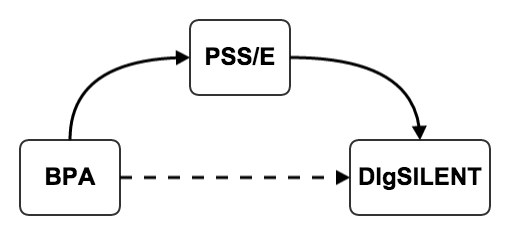
\includegraphics[width=0.7\textwidth]{images/Paper_Fig_11.png}
\setcaptionwidth{\linewidth}
\caption{BPA、PSS/E、DIgSILENT数据转换研究现状示意图}
\end{figure}

如图1.1所示,在之前的研究中,转换BPA数据至PSS/E数据的程序已经比较成熟,同时PSS/E至DIgSILENT的转换也得到了较好地实现,因此之前主要是通过PSS/E为中介来从BPA数据转换到DIgSILENT,这样就带来很大的不便。在BPA数据不经过PSS/E直接转换到DIgSILENT方面,杨迪行学长通过DIgSILENT自带的DPL语言实现了其转换,但DPL语言实用性不强,在诸多方面不及Python应用灵活、功能强大,在新版本的DIgSILENT中新加入了Python的API接口,也为这种实现提供了可能性。

\section{项目研究的主要内容}

本项目基于DIgSILENT平台,致力于研究从BPA到DIgSILENT的数据转换问题:将BPA的数据导入DIgSILENT中,利用Python语言编程,实现从外部数据的读取,并且将读到的数据在DIgSILENT中建立相应的模型并予以赋值,从而在DIgSILENT得到与BPA中相同的数据模型,进而可以利用两个软件不同的优势进行数据的计算。
论文的工作主要从以下几个方面展开:
\begin{itemize}
\item 对Python在DIgSILENT中的API接口进行介绍,分析其在BPA至DIgSILENT数据转换的应用和功能方面的优势。
\item 对DIgSILENT和BPA数据的介绍。分别对DIgSILENT和BPA的数据特点进行具体的介绍,包括发电机模型,负荷模型等在两个不同软件的不同特点。
\item 从DIgSILENT里找到BPA软件中数据对应的模型及其参数位置。
\item 用Python语言进行编程,将外部数据所代表的模型意义完全的在DIgSILENT中重现出来,即在DIgSILENT中重新建立模型,并赋予响应的参数值。建立他们之间的关系。
\end{itemize}

\begin{thebibliography}{99} % Bibliography - this is intentionally simple in this template

\bibitem{1}刘庆, 张东英, 刘燕华, 等. BPA 电网模型自动导入 DIgSILENT 的研究和开发[J]. 电力系统保护与控制, 2014, 42(16): 112-117.

\bibitem{2}李广凯, 李庚银. 电力系统仿真软件综述[J]. 电气电子教学学报, 2005, 27(3): 61-65.

\bibitem{3}吕涛, 韩祯祥. 电力系统仿真软件 DIgSILENT 介绍[J]. 华东电力, 2005, 32(12): 37-41.

\bibitem{4}吕涛. 电力系统仿真软件的运用与比较[M]. 浙江大学, 2005.

\bibitem{5}马龙义. BPA与PSS/E仿真模型分析与转换研究[D]. 华南理工大学, 2010.

\bibitem{6}马龙义, 武志刚, 侯冠基, 等. BPA 与 PSS/E 的暂稳态模型比较和数据转换[J]. 电力系统及其自动化学报, 2010, 22(5): 128-134.

\bibitem{7}PowerFactory. User's Manual DIgSILENT PowerFactory. Version 14.0 DIgSILENT GmbH. Gomaringen, Germany July 2010. Publisher: DIgSILENT GmbH. 

\bibitem{8}李东东, 王凯凯, 叶辰升. 采用双馈机组的风电场无功功率控制研究[J]. 电力系统保护与控制, 2013, 41(13): 37-42.

\bibitem{9}付超, 朱凌, 王慧, 等. 风电场并网在线预警系统研究[J]. 电力系统保护与控制, 2011, 39(17): 64-69.

\bibitem{10}苑国锋, 李永东, 柴建云, 等. 1.5 MW 变速恒频双馈风力发电机组励磁控制系统试验研究[J]. 电工技术学报, 2009, 24(2): 42-47.

\end{thebibliography}
